\documentclass{trkut}% Reaalkooli vormistus. Muidu "report" või "article".
\usepackage[style=trkut]{biblatex}% Kasutatud kirjanduse genereerimine
\usepackage{pgfplots}
\usepackage{amsmath}
\usepackage{siunitx}
\usepackage{wasysym}
\usepackage{verbatim}
\usepackage{listings}
\addbibresource{viited_eesnimi_perekonnanimi.bib}% Viidete info fail
\defbibheading{bibliography}{\addchap{#1}}% Lisame kasutatud materjalid sisukorda

\pealkiri{Atmosfääri mudeldamine ja katseandmete põhjal täpseima mudeli leidmine} % Kahel real
\autor{Jarl Patrick Paide}
\klass{11.a}
\juhendaja{õp Mart Kuurme } %\\ õp Kaarel Kivisalu}% Toetab praegu ainult ühte juhendajat, manual fix: muuda cls failis juhendaja -> juhendajad

\begin{document}
\maketitle% Tiitelleht
\tableofcontents% Sisukord

\addchap{Sissejuhatus}
\nummerdame% See käsk peab olema kohe peale sissejuhatust
%See teema on aktuaalne, kuna see on väga huvitav ja ma tahan seda uurida...
Globaliseeruvas ja ülerahvastatud maailmas on maa atmosfääri reostatus üks kõige olulisemaid probleeme. Atmosfääri reostusega kaasneb kasvuhooneefekt - kliima soojenemine, mis omakorda viib maailmamere tõusule. Atmosfääri mudeldamine aitab mõista atmosfääris toimuvaid protsesse ja leida lahendusi atmosfääri seisundi parandamiseks. Mudeli andmeid saab kasutada globaalse atmosfääri mudeli väljatöötamisel.

Uurimistöö eesmärk on leida vaatlusandmete alusel võimalikult täpne mudel, mis kirjeldaks atmosfääri temperatuuri ja rõhu seoseid vastavalt kõrgusele maapinnast. Uurimisküsimus on "Millised seosed on atmosfääris mõõdetavate parameetrite vahel - temperatuur, rõhk ja kõrgus maapinnast?".

Uurimistöö alguses leitakse erinevate eeldustega erinevad seosed temperatuuri ja rõhu sõltuvusest kõrgusest. Praktilises osas tehakse mõõtmisi heeliumõhupalli külge kinnitatud mõõteriistaga, mis lennutatakse stratosfäärini ja pärast kontrollitakse katseandmete põhjal teoreetilises osas saadud seoste kehtivust.





\chapter{Teooria}
Käesolevas osas leitakse seoseid, kuidas kirjeldada atmosfääris rõhu ja temperatuuri sõltuvust kõrgusest.

\begin{figure}[h]
	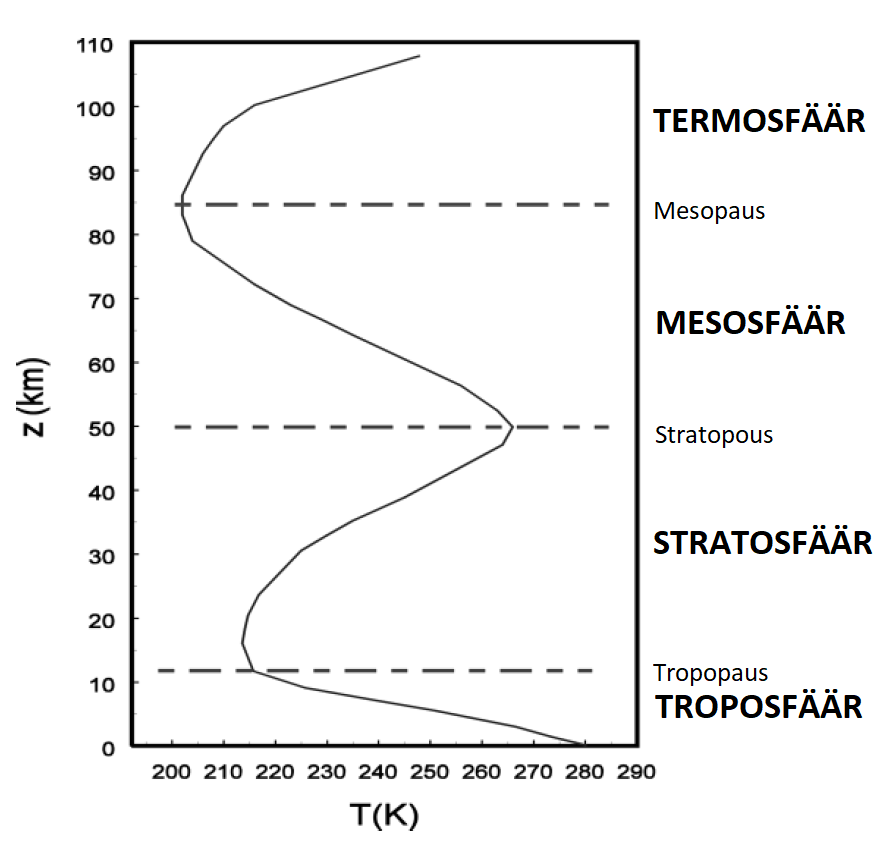
\includegraphics[width=0.5\textwidth]{PicGra/Profile2.png}
	\caption{Temperatuuri sõltuvus kõrgusest}
	\allikas{\cite{book:779878}}
	\label{profile}% Selle järgi viidatakse, see rida peab olema pärast \caption
\end{figure}

Joonisel \ref{profile} on näha, kuidas temperatuur muutub kõrguse kasvades. Troposfääris temperatuur langeb ja stratosfääris temperatuur tõuseb. Kõrguse kasvades rõhk väheneb, sest kõrguse kasvades väheneb ülevalpool oleva õhu mass, mis surub õhku kokku, tekitades rõhku. Kuna rõhk väheneb, siis temperatuur langeb. See seletab temperatuuri langust troposfääris. Peale troposfääri tuleb osoonikiht, mis asub stratosfääris. Osoon neelab päikeselt tulevat kiirgust, muutes selle soojuseks. Mida kõrgemal, seda vähem kiirgust on neelatud päikese poolt ja seda soojem. Eelkirjeldatud atmosfääri kihtides on kogutud käesoleva uurimistöö katseandmed.

On olemas erinevaid gaasi mudeleid. Nendest kõige tuntum on ideaalse gaasi olekuvõrrand. Ideaalne gaas erineb reaalsest gaasist kahe eelduse poolest. Ideaalses gaasis ei arvestata osakeste vahelist vastastikjõude. Ideaalses gaasis on osakestel tühiselt väike suurus. Võib eeldada, et gaas on ideaalne siis, kui rõhk on väike kriitilise rõhu suhtes ja temperatuur on kõrge kriitilise temperatuuri suhtes. Kui rõhk on kõrge, siis on osakestevahelisi kokkupõrkeid palju ja osakeste suurus saab oluliseks. Kui temperatuur on madal, siis liiguvad osakesed aeglaselt ja osakestel on rohkem aega olla üksteise mõjuväljas ja saada mõjutatud. Kui vaadata atmosfääri, siis kõige kõrgem rõhk on maa lähedal ja kõrguse suurenedes see väheneb, millega väheneb ka osakeste vaheline vastasmõju. Atmosfääris olevad rõhud on väikesed, võrreldes õhu kriitilise rõhuga. Temperatuur võib langeda atmosfääris küll madalale, aga mitte piisavalt madalale, et see läheneks kriitilisele temperatuurile. Seega võib eeldada, et atmosfääris olevad gaasid käituvad kui ideaalsed gaasid. Ideaalse gaasi olekuvõrrand on:
\begin{equation}\label{eq8}
pV=\nu RT ,
\end{equation}
kus $p$ on gaasi rõhk, $V$ on gaasi ruumala, $\nu = \frac{m}{\mu}$ on gaasi kogus moolides, kus $m$ on gaasi mass ja $\mu$ on gaasi molaarmass, $R$ on univarsaalne gaasikonstant ja $T$ on gaasi temperatuur.

Atmosfääris rõhk langeb kõrguse kasvades. Rõhu erinevus erinevatel kõrgustel toob kaasa rõhkude vahest tingitud ülespoole suunatud jõu, mida tasakaalustab gravitatsiooni jõud. Rõhk muutub $dp$ võrra kõrguse $dz$ võrra kasvades, kui õhu tihedus kõrgusel $z$ on $\rho$, järgnevalt:
\begin{equation}\label{eq10}
dp=-\rho gdz.   
\end{equation}


\section{Adiabaatiline protsess}
Termodünaamika esimene seadus on
\begin{equation}\label{eq1}
dU = dQ - dA
\end{equation}
kus $dU$ on gaasi siseenergia muutus, $dQ$ on soojushulga muutus ja $dA$ on töö muutus. Gaasi siseenergia $U$ avaldub vabadusastmete $i$ kaudu järgneva seose abil:
\begin{equation}\label{eq5}
U = \frac{i}{2} \nu R T.
\end{equation}
Konstantse ruumala puhul tööd ei tehta, seega kogu soojus läheb siseenergia suurendamiseks. Saame soojusmahutavuse, võttes siseenergia muudust tuletise temeratuuri järgi:
\begin{equation}\label{eq6}
C_V = \frac{dQ}{dT}=\frac{i}{2}\nu R
\end{equation}
Molaarset soojusmahutavust saab avaldada valemiga $c_V = \frac{C_V}{\nu}$, saades molaarseks soojusmahutavuseks
\begin{equation}\label{eq7}
c_V = \frac{i}{2}R.
\end{equation}
Kui aga vaadata isobaarilist protsessi, siis olekuvõrrandist tuleneb: $pdV=\nu RdT$, ning gaas teeb tööd $dA = pdV = \nu RdT$. Avaldades need valemisse \ref{eq1} saadakse:
\begin{equation*}
dQ = dU + dA = \frac{i+2}{2} \nu R dT
\end{equation*}
millest järeldub:
\begin{equation*}
c_p=\frac{i+2}{2}R.
\end{equation*}
Samuti saab näidata $c_V$ ja $c_p$ vahelist seost:
\begin{equation}\label{eq9}
c_p = c_V + R.
\end{equation}
Adiabaatiline protsess on termodünaamiline protsess, mille käigus ei toimus soojusvahetust väliskeskkonnaga. Kuna adiabaatilises protsessis soojusvahetust ei toimu, siis valemis \ref{eq1} $dQ=0$. Gaasi poolt tehtud töö on $d A=pdV$ ja gaasi siseenergia muut on $dU=\nu c_VdT$. Sellest järeldub:
\begin{equation}\label{eq2}
\nu c_VdT = -pdV.
\end{equation}
Ideaalse gaasi olekuvõrrandist \ref{eq8} saadekse tuletist võttes ja avaldades järgneva seose:
\begin{equation}\label{eq3}
dT = \frac{pdV+Vdp}{\nu R}.
\end{equation}
Asendades \ref{eq3} valemi valemisse \ref{eq2} saadakse uus seos:
\begin{equation}\label{eq4}
pdV(c_V+R)+c_VVdp=0.
\end{equation}
Asendame siia sisse valemi \ref{eq9} ja adiabaadi näitaja $ \gamma \equiv \frac{c_p}{c_V}$ saadakse võrrand
\begin{equation*}
\gamma \frac{dV}{V} + \frac{dp}{p} = 0.
\end{equation*}
Seda integreerides saadakse uus võrdus:
\begin{equation*}
 \int \gamma \frac{dV}{V} + \frac{dp}{p} = \gamma \ln(V) + \ln(p) = Const.
\end{equation*}
Sellest saab järeldada
\begin{equation*}
pV^\gamma = Const.
\end{equation*}
Samuti kasutades ideaalse gaasi olekuvõrrandid saab tuletada järgneva seose:
\begin{equation}\label{eq13}
p^{1-\gamma}T^\gamma = Const.
\end{equation}
Seega adiabaatilise protsessi puhul ei muutu antud võrrandi väärtus-

\section{Kuiv adiabaatiline temperatuurigradient }
Harilikult on õhumassid atmosfääris tugevas liikumises, nii et nad liiguvad pidevalt üles-alla. Kuna kõrgemal on rõhk väiksem kui all, siis jahtub gaas üles liikudes adiabaatilise paisumise tõttu (õhumasside suurte mõõtmete tõttu on soojusjuhtivus hästi aeglane). Selles osas vaadatakse olukorda, kui õhk on täiesti kuiv.

Valemist \ref{eq13} saadakse
\begin{equation*}
d\ln(p^{1-\gamma}T^\gamma) = 0,
\end{equation*}
millest saadakse
\begin{equation}\label{eq17}
\frac{dp}{p} = \frac{\gamma}{\gamma-1}\frac{dT}{T}.
\end{equation}
Asendades seos \ref{eq10} seosesse \ref{eq17} saadakse temperatuuri gradiendi:
\begin{equation}\label{eq11}
\Gamma \equiv \frac{dT}{dz}=-\frac{\gamma-1}{\gamma} \frac{\mu g}{R} = -\frac{R}{c_p}\frac{\mu g}{R} = -\frac{\mu g}{c_p}.
\end{equation}


\section{Märg adiabaatiline temperatuurigradient}
Valem \ref{eq11} töötab juhul, kui õhus pole vee auru. Kui õhus on vee aur ja see pole küllastunud toimuvad atmosfääris ikkagi adiabaatilised protsessid. Sellisel juhu kehtiv valem 
\begin{equation*}
\Gamma = -\frac{\mu g}{c_p}
\end{equation*}
kus $c_p$ on õhu ja vee auru erisoojuse summa, saades lõpplikuks valemiks
\begin{equation*}
\Gamma = -\frac{\mu g}{(1-\omega)c_{p,o} + \omega c_{p,v}}
\end{equation*}
kus $c_{p,o}$ on õhu erisoojus, $c_{p,v}$ on vee auru erisoojus ja $\omega$ on vee hulgaosakaal.

\section{Rõhu muutus kõrgusega }
Integreerides valemit \ref{eq10} saadakse
\begin{equation*}
\int_{T_0}^{T} dT = \int_{0}^{z} \Gamma dz
\end{equation*}
\begin{equation*}
T-T_0 = \Gamma z,
\end{equation*}
kus $T_0$ on temperatuur algpunktis ja $T$ on temperatuur kõrgusel $z$ algpunktist. Avaldist ümber paigutades saadakse:
\begin{equation*}
T = T_0 \left(1+\frac{\Gamma}{T_0}z\right).
\end{equation*}
Kasutades nüüd seost \ref{eq13}, saab eelmise valemi ümber kirjutada kujul:
\begin{equation*}
p=p_0 \left(1+\frac{\Gamma}{T_0}z\right)^{\frac{\gamma}{\gamma-1}}.
\end{equation*}
Astendaja saab asendada kujuga
\begin{equation*}
\frac{\gamma}{\gamma-1} = \frac{c_p}{R} = -\frac{g\mu}{\Gamma R},
\end{equation*}
saades lõplikuks valemiks:
\begin{equation*}
p=p_0 \left(1+\frac{\Gamma}{T_0}z\right)^{ -\frac{g\mu}{\Gamma R}}.
\end{equation*}
Seega kui on teada algpunktis olev rõhk $p_0$, temperatuur $T_0$ ja temperatuurigradient $\Gamma$ on võimalik leida seda valemit kasutades rõhk kõrgusel $z$ algpunktist. Kui asendada siia valemisse kuiva õhu temperatuurigradient \ref{eq11} saadakse
\begin{equation*}
p=p_0 \left(1-\frac{\gamma-1}{\gamma}\frac{\mu g}{RT_0}z\right)^{\frac{\gamma}{\gamma-1}}.
\end{equation*}
Kuid see valem töötab ainult kuiva õhu puhul.



\section{Pilved}
Kui niiske õhk tõuseb kõrgemale, siis väheneb temperatuur ja rõhk. Kui õhk jahtub ja rõhk väheneb, siis väheneb ka õhu võime hoida vett auruna endas ja vesi kondenseerub väga väikesteks tilkadeks. Veel on lihtsam kondenseeruda, kui vesi saab kondenseeruda osakese külge. Nendeks osakesteks on tavaliselt tolm, õietolm või muud sellist. Kui piisavalt palju vett kondenseerub väikeste osakeste külge, siis moodustub pilv.

Adiabaatiline protsess on termodünaamiline protsess, mille käigus soojusvahetust ei toimu. Pilvedes vee kondenseerumisel eraldub soojus, seega pilvedes toimuv termodünaamiline protsess ei vasta adiabaatilisele protsessile. Kuid adiabaatiline protsess töötab niiske õhu puhul madalamal ja kõrgemal pilvede kõrgusest, kuna soojusvahetust pole.

Järgnevalt leitakse suhe välja aurustunud vee ja õhu vahel. Temperatuuri gradient vahetult pilve all on $\Gamma$, temperatuur pilve all on $T_0$, temperatuur pilvede kohal $z$ võrra kõrgemal algtemperatuurist on $T_2$, vaadeldava õhu mass on $m_a$ ja sellest õhust kondenseerunud õhu vee mass on $m_v$. Kui pilvi ei oleks, siis muutuks temperatuur edasi vastavalt temperatuuri gradiandile. Seega temperatuur oleks $T_2$ asemel
\begin{equation*}
T_1 = T_0 + \Gamma z.
\end{equation*}
Vesi annab kondenseerumisel ära energia
\begin{equation*}
\Delta U = L m_v
\end{equation*}
kus $L$ on keemisenergia. See energia läheb õhu siseenergia suurendamiseks
\begin{equation*}
\Delta U = \frac{i}{2}\frac{m_a}{\mu}R\left(T_2 - T_0 - \Gamma z\right).
\end{equation*}
Seega vett eraldub ühest ühikmassist õhust pilvedes
\begin{equation*}
\frac{m_v}{m_a} = \frac{i}{2}\frac{R}{\mu L}\left(T_2- T_0 - \Gamma z\right).
\end{equation*}


\section{Päikese mõjutus}
Peale troposfääri tuleb stratosfäär. Startosfääris temperatuur suureneb kõrguse kasvades. See on tingitud päikeselt tuleneva valgusenergia neeldumisest osoonikihis ja soojusena eralduv energia soojendab õhku. Kuna siseenergiat antakse õhule juurde, siis pole tegu enam adiabaatilise protsessiga. Järgneatl arvutatakse, kui palju suureneb õhu siseenergia atmosfääris. Temperatuur enne stratosfääri sinenemist on $T_0$ ja temperatuuri gradient samal kõrgusel on $\Gamma$. Temperatuur $z$ võrra kõrgemal stratosfääris on $T_2$. Kui päikest ei paistaks, siis temperatuur langeks edasi temperatuuri gradiendi järgi. Seega sellisel juhul oleks temperatuur $z$ võrra kõrgemal algpunktist
\begin{equation*}
T_1 = T_0 + \Gamma z.
\end{equation*}
Siseenergia avaldub kujul:
\begin{equation*}
U = \frac{i}{2}\gamma RT.
\end{equation*}
Seega on siseenergia 
\begin{equation*}
\frac{U_2}{U_1} = \frac{\frac{i}{2}\gamma RT_2}{\frac{i}{2}\gamma R\left(T_0 + \Gamma z\right)} = \frac{T_2}{T_0+\Gamma z}
\end{equation*}
korda suurem sellel kõrgusel päikesega kui ilma päikesega.





\chapter{Katse ülesehitus}
Katse käigus mõõdeti atmosfääris, troposfääris ja stratosfääri madalamates kihtides rõhku, temperatuuri ja õhuniiskust. Selle jaoks kasutati heeliumõhupalli külge kinnitatud sondi, mis tegi mõõtmisi. Andmeid koguti heeliumiga täidetud õhupalliga kaasa saadetud sondiga, mis mõõtis erinevaid andmeid.

Põhilisteks andmeteks on kõrgus, asukoht, aeg, välistemperatuur ja rõhk. Sondi pardal oli Raspberry Pi arvuti. Õhupall kerkib atmosfääri kõrgemadesse kihtidesse, sest üleslükkejõud ületab kerge gaasi ja sondi massi. Kõrgemale tõustes rõhk väheneb. Et õhupalli siserõhk oleks tasakaalus välisrõhuga, suureneb õhupalli ruumala, kuni õhupall lõhkeb ülepingest. Peale seda kukkub sond alla ja leitakse GPS'ga üles.


\section{Katse eesmärk}
Katsel oli kaks eesmärki. Üks eesmärk oli käesoleva uurimistöö jaoks koguda atmosfäärist andmeid, et testida reaalsete katseandmete kokkulangemist teoreetiliselt tuletatud valemitega. Teiseks tekkis idee tuua midagi atmosfäärist kaasa ja see idee suunati edasi Reaalkooli põhikooli õpilastele, kes arendasid ideed edasi ja otsustasid stratosfäärist õhku läbi filtri juhtida ja sellega koguda stratosfäärist tolmu ja muid suuremaid osakesi. Tolmu kogumine ei käi selle uurimistöö juurde.

Esimeses petükis koostatud mudeli kontrollimiseks oli vaja koguda atmosfääri erinevatest kõrgustest andmeid temperatuuri, rõhu ja õhuniiskuse kohta.

\section{Katsemetoodika valik}
Selles uurimistöös tehtud katsed on tehtud koostöös Eesti kosmosekoolide võrgustikuga.

Eesti kosmosekoolide võrgustik oli enne selle uurimistööga tehtud lendu teinud kaks lendu. Esimene lend mis tehti 29. märtsil 2018 kestis umbes kaks tundi, kus kõrgeim punkt milleni jõuti oli \SI{26474}{m}. Selleks läks aega poolteist tundi. Kokku tehti 220 mõõtmist. Mõõtmise alla kuulusid kellaaeg, laiuskraad, pikkuskraad, kõrgus, kapsli sisetemperatuur, välistemperatuur ja rõhk. Teine lend tehti 11. mail 2018 ning seekord kestis lend peaaegu neli tundi, jõudes kolme ja poole tunniga kõrgusele \SI{32608}{m}. Katse tegijad muutsid õhupallis heeliumi kogust, mille tõttu oli tõusmise kiirus väiksem, aga õhupall plahvatas hiljem ja jõuti kõrgemale. Seekord tehti 4300 mõõtmist ja mõõdeti samu parameetreid.

Katse korraldamiseks ja läbiviimiseks vajalikud oskused saadi Eesti kosmosekoolide võrgustiku poolt korraldatavast koolituselt ja sealt on pärit vastav metoodika.

\section{Katse planeerimine}
Alguses oli plaanis lendu teha Väätsa staadionilt, aga kasutades http://predict.habhub.org/ lehel olevat kalkulaatorit, oli ennustusest näha, et sond oleks kukkunud Jõhvi lähedale. Kuna eksimusruum võib olla suur ning Venemaa piir ja meri ei olnud kukkumiskohast kaugel, siis otsustati lennu start teha võimalikult edelast nii, et edelatuultega kalduks sond Kesk-Eestisse. Rihtides lõppsihtkohta Paide peale, otsustati start teha Varblast Pärnumaalt.

Lennu jaoks oli vajalik saada lennuametilt kooskõlastus.

Sondi ehitamise eest vastutasid Tallinna Reaalkooli põhikooli õpilaste robootikameeskond Viirus. Sondi põhiehitusmaterjaliks oli penoplast ja puidust tikud. Sond pidi hoidma sisetemperatuuri madalate välistemperatuuride eest, et sisemuses olev elektroonika töötaks. Samuti pidi korpus vastu pidama kukkumisele ning kõige juures pidi korpus olema võimalikult kerge. Selle tõttu valiti korpuse materjaliks penoplast ja tikud. Kuna ühe lennuga saab üles saata mitu katset, siis otsustas põhikooli õpilaste meeskond Viirus koguda atmosföörist tolmu tõmmates õhku läbi filtri. Tolmu sooviti koguda võimalikult kõrgelt. Ennustuse kohaselt oleks pidanud sond lendama \SI{27}{km} kõrgusele, kuid kuna sondi mass ületas planeeritud massi, siis arvati, et sond väga kõrgele ei lenda ja väikese lisavaruga arvestades määrati vahetult enne starti tolmukogumise alustamise kõrguseks \SI{20}{km}.

Sondi sees olev ruum oli jaotatud kaheks. Alumises olid kaks toru, mis olid parralleelsed ja läbisid sondi kere. Nenede sees olid klapid, ventilaator ja filtrid. Ülemises osas oli kogu tehnika. Mõõtmisi tegi ja klappe avas Raspberry Pi arvuti. Voolu andis nii ventilaatoritele kui ka Raspberry Pi'le akupank. Raspberry Pi külge oli kinnitatud raadioantenn, GPS-antenn mootor klappide jaoks ja andur BME280, mis mõõtis õhu rõhku, temperatuuri ja õhuniiskust.
\begin{figure}[h]
	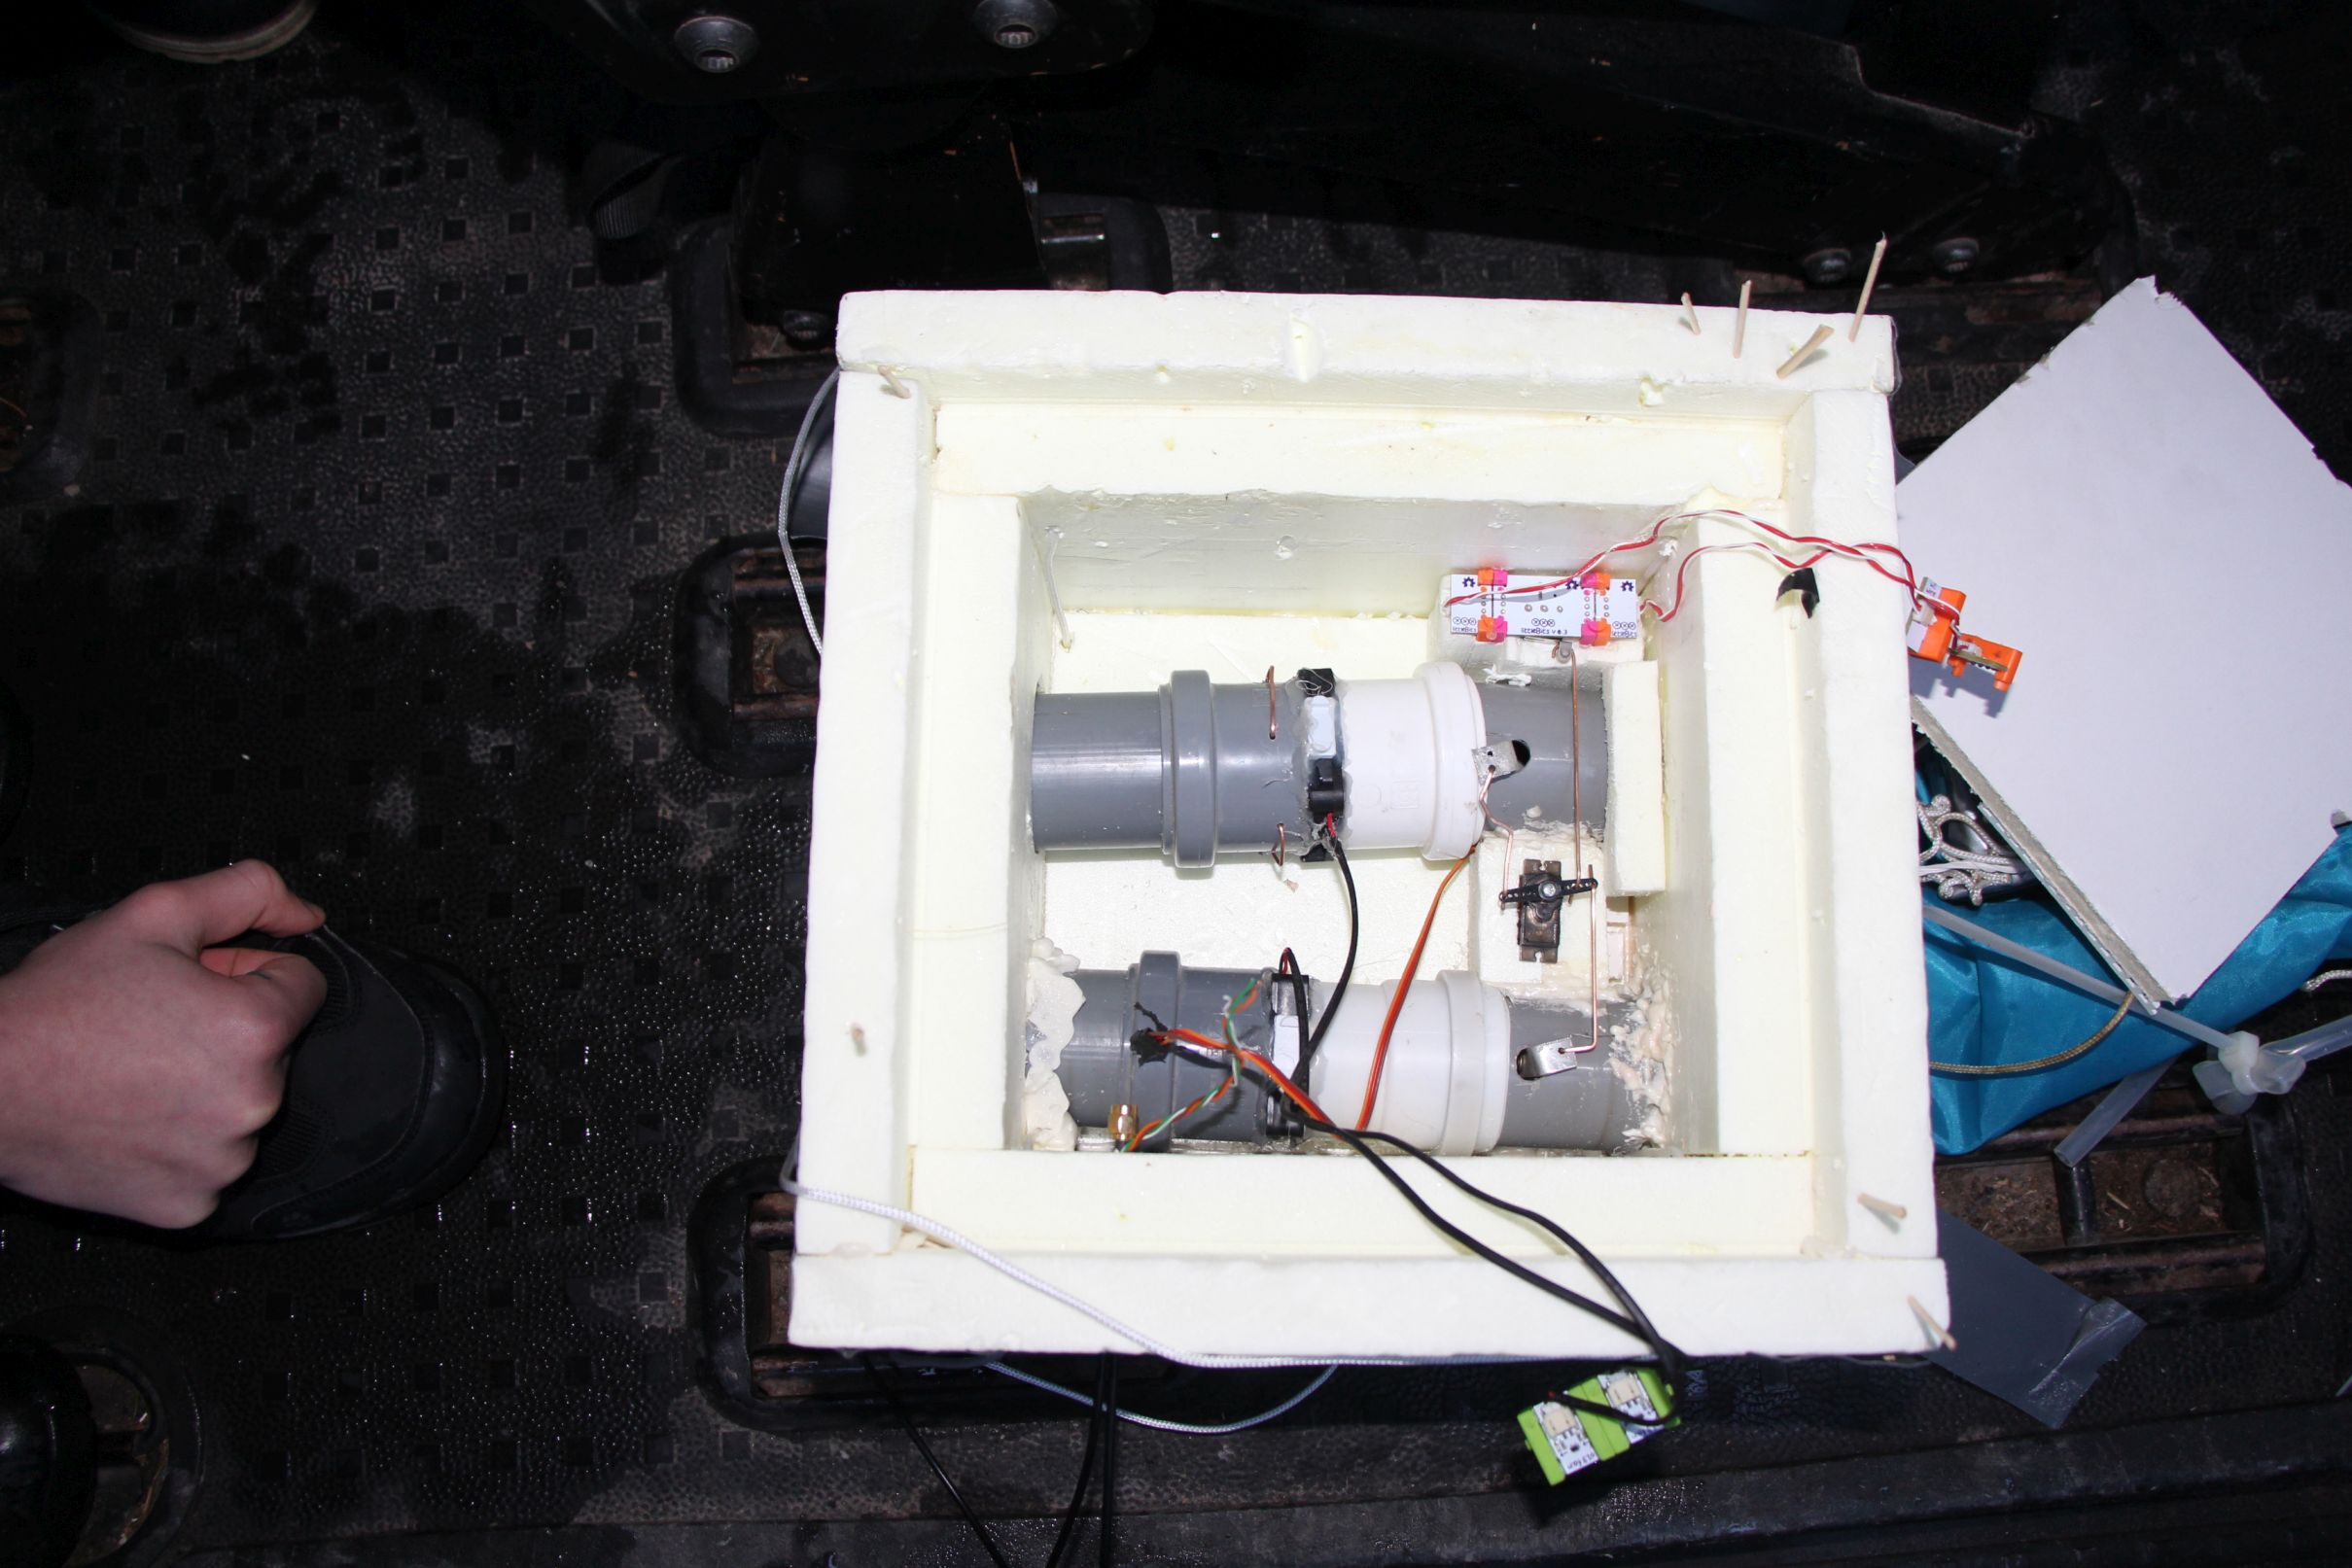
\includegraphics[width=1\textwidth]{PicGra/sond2korrus.jpg}
	\caption{Pilt sondist}
	\allikas{\url{http://pildid.real.edu.ee/main.php?g2_itemId=84935}}
	\label{sond1}
\end{figure}

Sondi mass oli \SI{1375}{g}. Sondi korpus oli ehitatud, kasutades penoplasti ja puittikke. Sondist tuli välja nii raadio kui ka GPS-antenn ning ka andur BME280. Sondi peale oli kinnitatud langevari. Eraldi korpuses asus GPS tracker GL300 mida kasutati pärast sondi leidmisel. Lennuks kasutati Hwoyee \SI{600}{g} õhupalli.
\begin{figure}[h]
	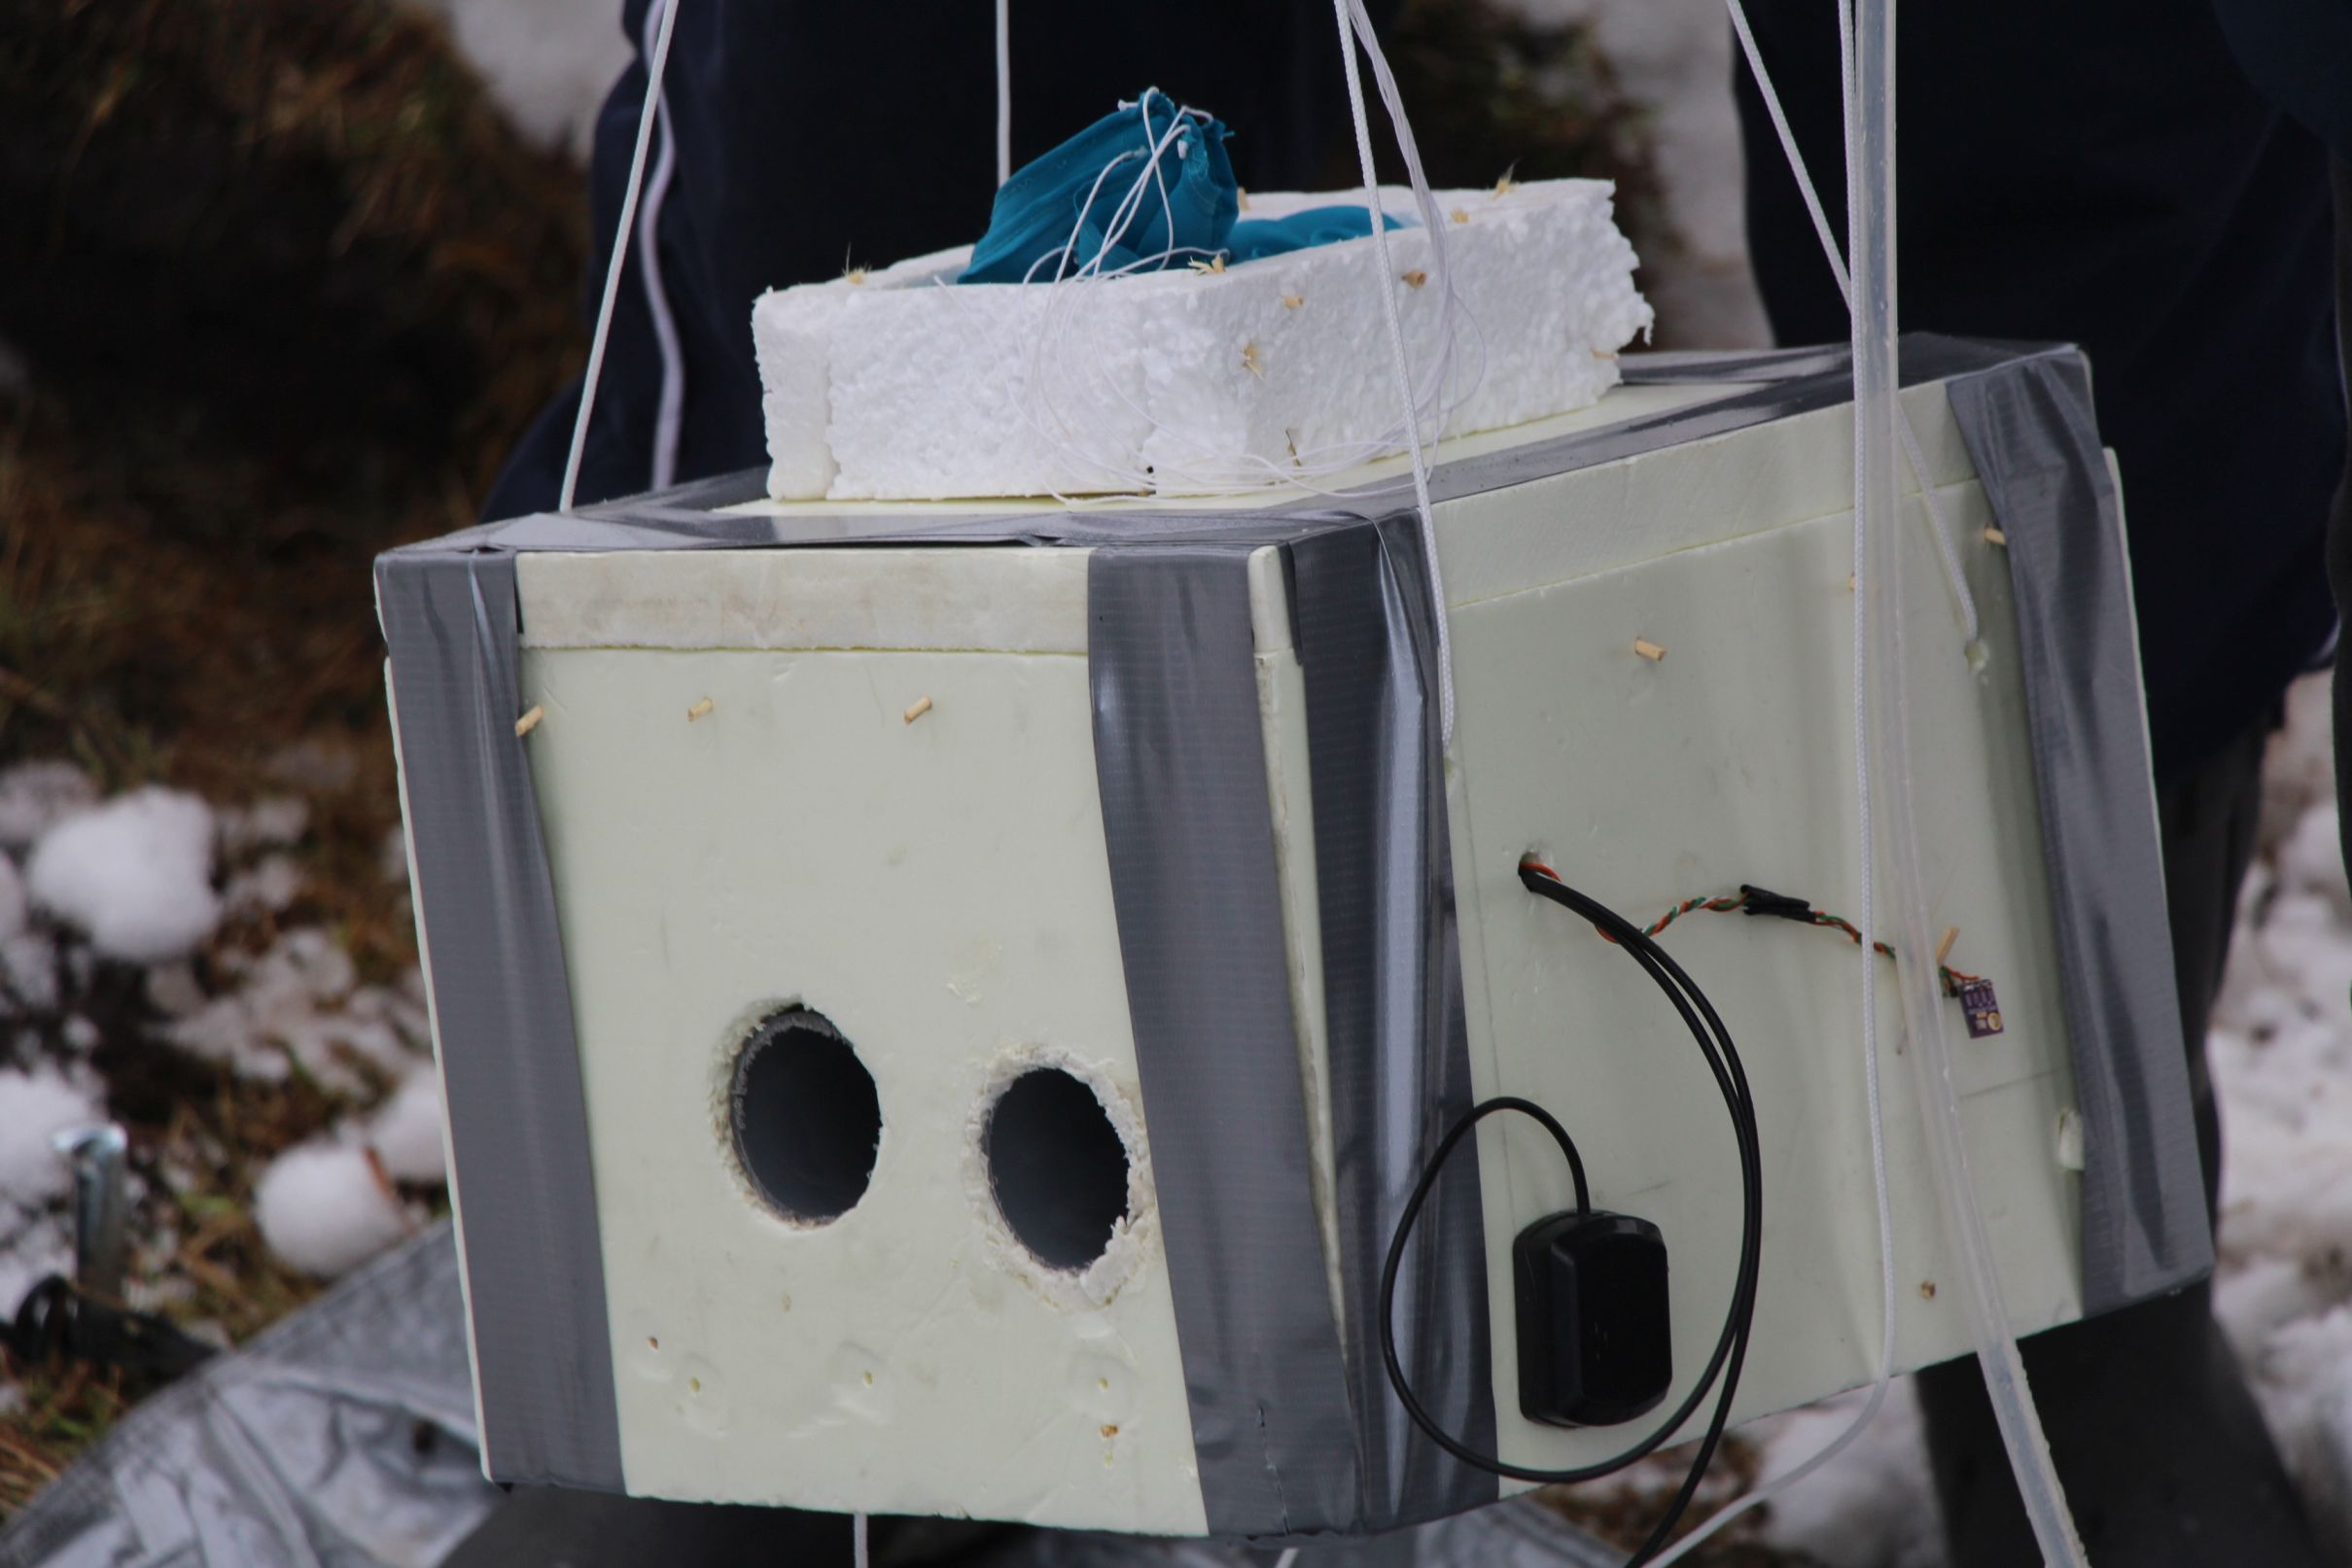
\includegraphics[width=0.5\textwidth]{PicGra/sond.jpg}
	\caption{Pilt sondist}
	\allikas{\url{http://pildid.real.edu.ee/main.php?g2_itemId=84935}}
	\label{sond2}
\end{figure}


\section{Katse seadmed}
Kogu tehnilist poolt juhtis Raspberry Pi arvuti. Raspberry külge kinnitati lisaks Pi In The Sky (PITS) plaat. PITS plaadi külge kinnitati GPS-antenn, mille järgi saadi teada geograafilisi koordinaate, kõrgust ja kellaaega, ja raadio antenn, millega saadeti mõõdetud andmed maapinnale, et jooksvalt jälgida sondi lendu. Raspberry Pi arvuti küljes oli temperatuuri andur, millega mõõdeti sisetemperatuuri. RP külge kinnitati BME280 sensor. Sensor mõõtis temperatuuri, õhurõhku ja õhuniiskust. Sennsor viidi juhtmetega sondist välja, et mõõta välistingimusi, mitte sondi sisetingimusi. RP külge kinnitati ka väike mootor. Mootori pööramisel avanesid klapid ja sulgus vooluring, millega pandi ventilaatorid tööle. Sondi sees on akupank, mis oli ühe juhtmega ühendatud RP külge toiteks ja teise juhtmega ühendatud vooluringi, kus asusuid ventilaatorid.

Andmeid kogus käesoleva uurimistöö autori poolt kirjutatud programm. Programm sai GPS'i kaudu teada andmed ja lisab sinna sensori poolt mõõdetud tulemused. Saadud andmerea salvestas programm logifaili ja lisaks saatis PITS plaadi külge kinnitatud raadioantenni kaudu info laiali. Programm kontrollis igal ajahetkel kõrgust ja kui see ületas soovitud kõrgust, saatis programm signaali moororile, pöörates mootorit. Kui kõrgus oli soovitust väiksem siis, pandi mootor tagasi algasendisse.

Raadiosignaal saadi kätte raadioantenniga, mille signaal edastati arvutisse. Kasutades tarkvaralist raadiot, muudeti saadud signaal heliks ja suunati virtuaalse helijuhtme abil helikaardi dekodeerimistarkvarra. Seal muuudeti heli tekstiks, kust oli võimalik välja lugeda mõõdetud andmed.

Eraldi väikessesse korpusesse pandi GL300 jälgija ja kinnitati suurema korpuse külge. Jälgija pandi eraldi korpusesse, et signaalid erinevate seadmete vahel ei hakkakse segama üksteist. Jälgija kasutab GPS'i et leida oma asukohta ja siis saadab selle mobiilset andmesidet kasutades Internetti, kust on võimalik teada saada jälgija asukohta. Seade pandi sondiga kaasa, et pärast maandumist lihtsalt sond üles leida. Kuna nõrk raadiosignaal ei levi hästi läbi metsa, siis raadiosignaali abil leida sondi üles maandumiskohast on aeganõudev. Kuid kuna teatud kõrgusel kaob ära mobiilne võrk, siis on võimalik sellist meetodit kasutades jälgida sondi lennu alguses ja lennu lõpus, kui sond on maa lähedal.

\section{Katse läbiviimine}
Lennu planeeritud start oli kell 11:00 10. veebruaril 2019. Libedad teeolud külevaheteedel pikendasid stardikohale jõudmise aega lükates starti edasi. Varblasse jõudes otsiti sobiv koht, kus oli ruumi ja lage ala ida suunas, et sondi oleks võimalik lennates kaua jälgida, kuna tugev tuul puhus läänest. Õhupalli täideti balloonis olevast heeliumiga. Balloonis oli \SI{4000}{l} heeliumi. Soovitud heeliumikogus mõõdeti ballooni küljes oleva rõhumõõdikuga. Lennus kasutati \SI{600}{g} lateksist õhupalli. Õhupalli täitmiseks võeti plastmassist pastaka toru korpus ja selle ümber mässiti tihedalt õhupalli suu. Kinnituseks kasutati nipukaid. Pastaka teise otsa ühendati voolik, mis oli ühendatud ballooniga. Pastakat kasutati, et oleks võimalik teha võimalikult tihe ühendus vooliku ja õhupalli vahel ilma, et sulguks heeliumi liikumine balloonist õhupalli. Peale õhupalli täitmist volditi voolik õhupalli lähedalt mitmekordselt kokku ja kinnitati see nipukatega. Seejärel lõigati voolik läbi. Lisaks kinnitati ka nöör sondi ja õhupalli vahel õhupalli suu külge ja kinnitati nipukatega. Kokku pandi õhupalli umbes \SI{2800}{l} heeliumi. Tugeva tuule tõttu pidi õhupalli väga maa lähedal täitma ja lisaks kätega õhupalli kinni hoidma. Lisaks enne lõplikku vooliku läbilõikamist kontrolliti, kas õhupall suudab sondi õhku tõsta ja hinnati tõstejõu piisavust.

Vahetult enne lendu helistati lennuametisse ja küsiti viimast kinnitust lennuks. Lennu start oli kell 11:51. Sond kadus pilvise ilma tõttu mõne minutiga vaateväljast. Raadiosidet suudeti hoida umbes \SI{20}{min}. Peale seda polnud võimalik puhast signaali kätte saada. Siis kadus GPS trackeri ühendus mobiilisideme teenuspakkujaga kõrguse tõttu. Peale sideühenduse kadumist hakati liikuma ennustatava maandumiskoha poole Paidesse. Peale maandumist ühendas GPS tracker ennast uuesti teenusepakkuja võrku ja saadi teada sondi kukkumise asukoht. Sond maandus kell 14:06 Paide lähedal paarkümmend meetrit Tallinn-Tartu maanteest. Sondi maandumisest saadi teada umbes \SI{15}{min} peale seda, kui kontrolliti sondi asukohta jälgija kaudu.






\chapter{Katseandmete analüüs}
Andmete analüüsimisks kasutatti autori poolt kirjutatud programmi. Programm aitas suurest andmekogust välja sorteerida vajalikud andmed ja kontrollida katseandmete kokkulangemist teoreetiliste seostega.

\section{Lennu asukohaline ülevaade}

\begin{figure}[h]
	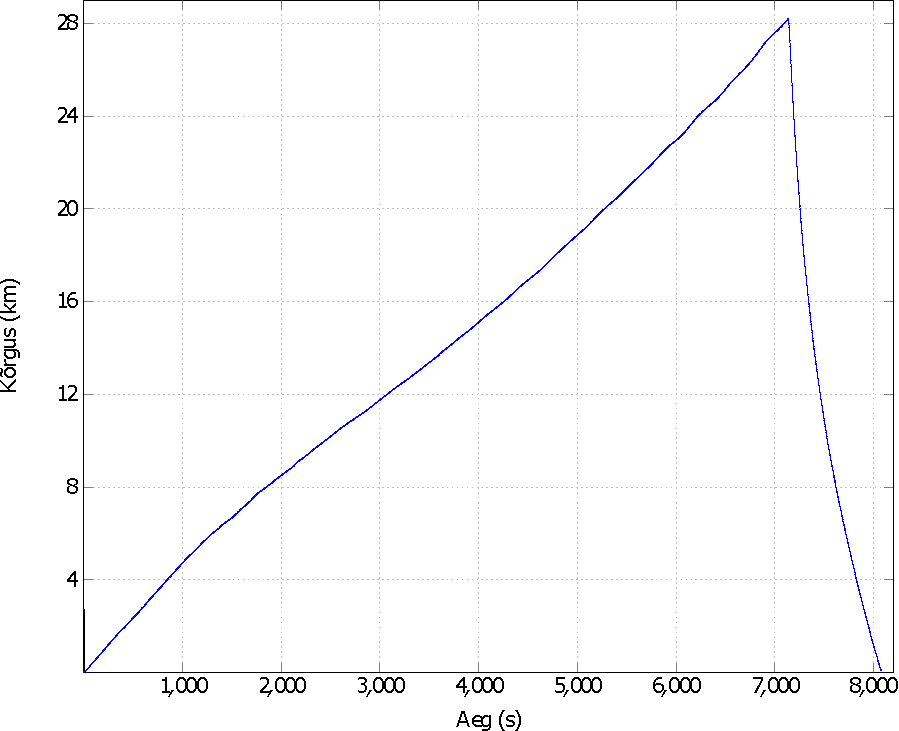
\includegraphics[width=1\textwidth]{PicGra/kõraeg.pdf}
	\caption{kõrguse sõltuvus ajast}
	%\allikas{Minu programm}
	\label{kõraeg}
\end{figure}

Joonisel \ref{kõraeg} on näha sondi kõrguse muutumist ajas. Kokku kestis lend \SI{8083}{sekundit}, ehk 2 tundi, 14 min ja 43 sekundit. Selle aja jooksul tehti kokku 2460 mõõtmist. Mõõtmised on tehut sekundilise täpsusega, eha kas iga 3 või 4 sekundi tagant. Keskmiselt tehti mõõtmisi iga \SI{3.29}{s} tagant.

Tõusmisel oli sondil ühtlane tõusukiirus. Keskmine kiirus tõustes oli \SI{3.95}{m/s}. Laskudes kiirus varieerus. Peale kukkumise algust langes sond kiiresti madala õhutiheduse tõttu. Keskmine kiirus peale langemise algust esimesel \SI{4}{km} oli \SI{78}{m/s}. Keskmine kiirus vahetult enne kokkupõrget maaga oli \SI{14}{m/s}. Kogu Kukkumise keskmine kiirus oli \SI{29.8}{m/s}.

\section{Temperatuuri muutus kõrgusega}
Joonisel \ref{TempKõrgus} on näha temperatuuri muutust kõrgusega. Joonisel on kaks joont, sest andmeid mõõdeti igalt kõrguselt kaks korda, sondi tõusmisel ja sondi laskumisel. Lennu stardi ajal oli kõrgem temperatuur kui lennu lõppemise ajal.

\begin{figure}[h]
	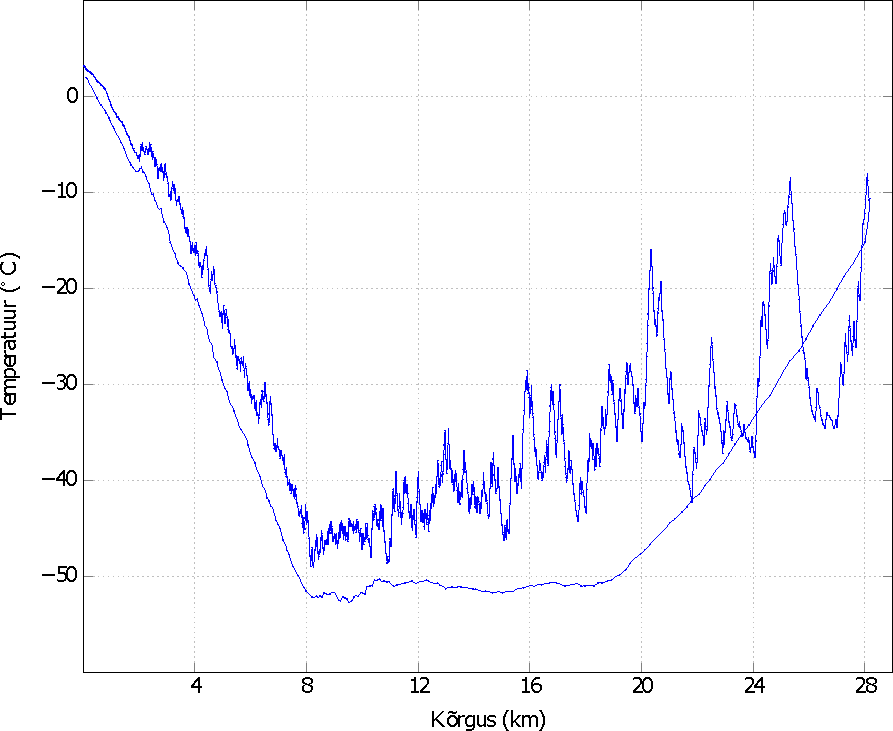
\includegraphics[width=1\textwidth]{PicGra/tempkõr.pdf}
	\caption{Temperatuuri sõltuvus kõrgusest}
	%\allikas{Minu programm}
	\label{TempKõrgus}% Selle järgi viidatakse, see rida peab olema pärast \caption
\end{figure}

Joonisel on näha, kuidas temperatuur kõigub, mitte ei muutu ühtlaselt. See on tingitud päikese kiirgusest. Kui sensor on päikese poole, siis soojendab päike sensorit. Kui sensor on sondi varjus, siis peale maha jahtumist mõõdab sensor jälle tegelikku õhutemperatuuri. Sensor ei mõõda kunagi madalamat temperatuuri tegelikust õhu temperatuurist. Kõrguse kasvades muutub temperatuuri kõikumise amplituud kõrgemaks. See on tingitud madalst rõhust. Kuna õhk hõreneb, siis hakkab sondi temperatuuri rohkem mõjutama päike kui õhk ise.

Kukkumine hakkab sel hetkel, kui sensor on ülesse soojenenud. Seega sensor kukkumise ajal jahtub, kuid kuna nende kõrguste juures kõrguse langemisel langeb ka temperatuur, ei saavuta sensor välisemperatuuri varem kui \SI{20}{km} kõrgusel maast. Sel ajal on näha sujuvat temperatuuri muutust. Sensori mitte ülessoojenemist kukkumisel võib põhjendada mitut moodi. Sond võis kukkumisel hakkata tugevalt pöörlema mille tõttu polnud sensoril aega üles soojeneda. Kogu lennu vältel oli sond külgtuultega samas kiiruse taustsüsteemis. Seega sondile mõjusid tuuled, mis tulevad üles liikumisest ja alla kukkumisest. Kuna kuni \SI{20}{km}'ni kukkus sond keskmise kiirusega \SI{70}{m/s}, siis jahutas tuul sensorit.

Kuna selles uurimistöös uuritakse täpsemalt tropsfääri osa, siis võib algul välja jätta kõik muud andmed mis on mõõdetud kõrgemal kui umbes \SI{8}{km}. Täpseks kõrguseks valiti \SI{8154}{m}. Sellel kõrgusel tehti viimane mõõtmine, mis oli temperatuurigraafiku viimane lokaalne miinimum, peale mida hakkas temperatuur jälle tõusma. Kuna graafik on ebatasane, vastab lokaalne miinimum kõige paremini tegelikkule temperatuurile. Sama kõrgus valiti ka kukkumisel.

Joonisel \ref{tempkõrtrop} on anomaalia. Umbes \SI{2}{km} kõrgusel on nii laskumisel kui ka tõusmisel näha kõrguse tõusmisega väikest temperatuuri muutust. Kuna see toimub nii tõusmisel kui ka kukkumisel siis on see suure tõenäelsusega tegelik temperatuuri muutus ja mitte sensori viga või muud sellist.
\begin{figure}[h]
	\includegraphics[width=1\textwidth]{PicGra/tempkõrtrop.pdf}
	\caption{Temperatuuri sõltuvus kõrgusest alla \SI{8}{km}}
	\allikas{Autori erakogu}
	\label{tempkõrtrop}% Selle järgi viidatakse, see rida peab olema pärast \caption
\end{figure}

Vaadates joonist \ref{humkõrtrop} on näha, et kuni \SI{2}{km} kõrguseni on õhuniiskus ühtlselt kõrge. Kuid peale \SI{2}{km} on näha, et õhuniiskus langeb tugevalt. Õhuniiskus langes, kuna sond väljus pilvedest, ning temperatuur tõusis. Pilvedest väljumist saab ka tõestada temperatuuri kõikumise algusega. Kuni \SI{2}{km}'ni temperatuur ei kõikunud, kuna päikest ei paistnud sondile peale. Pilvedest väljudes hakkas aga päike mõjutama sensori lugemist. Kuna osa mõõtmisi tehti pilvede sees ja osa pilvedest väljas, otsustati vaadelda temperatuuri muutumist eraldi pilvedest madalamal ja pilvedest kõrgemal.
\begin{figure}[h]
	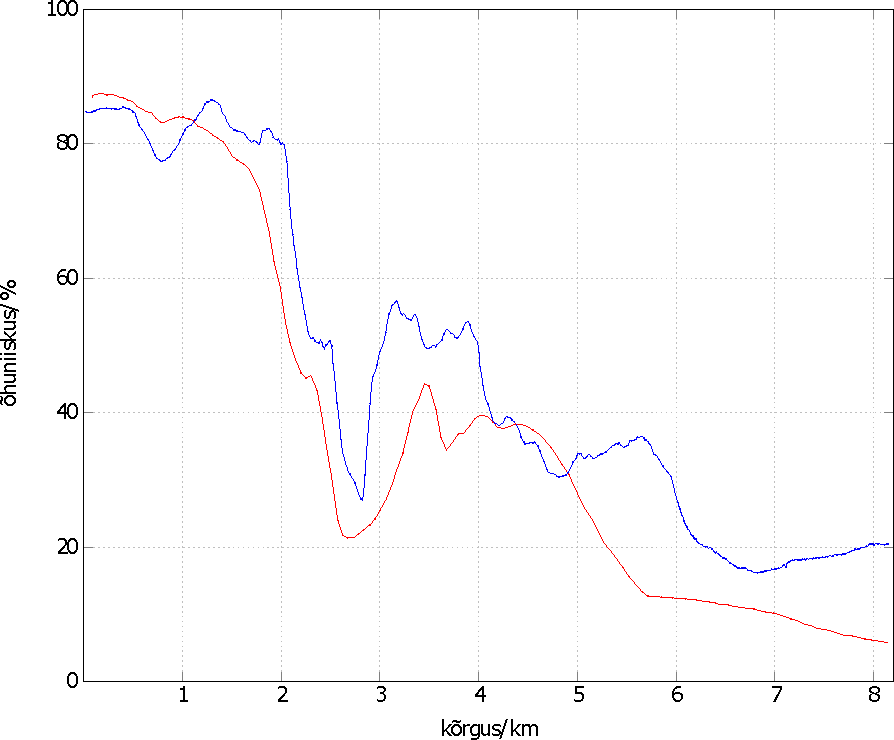
\includegraphics[width=1\textwidth]{PicGra/humkõrtrop.pdf}
	\caption{Õhuniiskuse sõltuvus kõrgusest alla \SI{8}{km}}
	\allikas{Autori erakogu}
	\label{humkõrtrop}% Selle järgi viidatakse, see rida peab olema pärast \caption
\end{figure}

Selles osas leitakse temperatuuri muutusele kõrgusega parim lineaarne seos:
\begin{equation*}
T(z) = T_0 + \Gamma z.
\end{equation*}
kus $T_0$ on temperatuur algpunktis ja $\Gamma$ on temperatuurigradient, ehk temperatuuri muutus kõrguse kasvades. Lineaarse seose leidmiseks kasutati vähimruutude meetodit, mis avalduv järgnevalt:
\begin{equation*}
\Gamma = \frac{\sum_{i=1}^{n}(z_i - \overline{z})(T_i - \overline{T})}{\sum_{i=1}^{n}(z_i - \overline{z})^2}
\end{equation*}
\begin{equation*}
T_0 = \overline{T} - \Gamma \overline{z}
\end{equation*}
kus $z$ on kõrgus ja $T$ on temperatuur.

Pilvede sees vaadati temperatuure õhupalli tõustes kuni \SI{2010}{m} meetrini. Sellel kõrgusel tehti viimane mõõtmine, peale mida temperatuur tõusis pilvedest väljumise tagajärgel. Samal põhjusel valiti laskumisel viimaseks andmepunktiks \SI{1926}{m} kõrgusel mõõdetud andmepunkt.

Joonisel \ref{tempkõrtroppilvlin} on näha temperatuuri muutust selles vahemikus. Laskumisel on temperatuuri gradient $\Gamma =  \SI{-5.53009}{\degreeCelsius/km}$ ning temperatuur algpunktis on $T_0 = \SI{2.12611}{\degreeCelsius}$. Tõusmisel esimese \SI{2}{km}'l on näha kahte erinevat lineaarset temperatuuri muutust. Esimesel \SI{793}{m}'l on temperatuuri gradient $\Gamma =\SI{-3.19233}{\degreeCelsius/km}$ ja temperatuur algpunktis $T_0 = \SI{3.16728}{\degreeCelsius}$. Kõrguste vahemikus \SI{808}{m} kuni \SI{2010}{m} on temperatuuri gradient $\Gamma =\SI{-5.73645}{\degreeCelsius/km}$ ja temperatuur algpunktis $T_0 = \SI{0.360244}{\degreeCelsius}$.

\begin{figure}[h]
	\includegraphics[width=1\textwidth]{PicGra/tempkõrtroppilvlin.pdf}
	\caption{temperatuuri sõltuvus kõrgusest alla \SI{2}{km}}
	\allikas{Autori erakogu}
	\label{tempkõrtroppilvlin}% Selle järgi viidatakse, see rida peab olema pärast \caption
\end{figure}


Tõusmisel valiti algpunktiks \SI{2565}{m} kõrgusel mõõdetud andmepunkt. See on esimene andmepunkt, alates \SI{2010}{m} kõrgusel asuvast andmepunktist, kus on madalam temperatuur, kui \SI{2010}{m} kõrgusel mõõdetud temperatuur. Laskumisel valiti algpunktiks \SI{2136}{m} kõrgusel mõõdetud andmepunkt. See on esimene andmepunkt, alates \SI{1926}{m} kõrgusel mõõdetud andmepunktist, kus on madalam temperatuur kui \SI{1926}{m} kõrgusel mõõdetud temperatuur. Antud vahemikus olevad mõõtmised on kuvatud joonisel \ref{tempkõrtroplin}.

Tõusmisel on temperatuuri gradient $\Gamma =\SI{-7.13399}{\degreeCelsius/km}$ ja temperatuur algpunktis $T_0 = \SI{-5.4533}{\celsius}$. Laskumisel oli temperatuuri gradient $\Gamma =\SI{-7.67992}{\degreeCelsius/km}$ ja temperatuur algpunktis $T_0 = \SI{-7.26635}{\celsius}$.

\begin{figure}[h]
	\includegraphics[width=1\textwidth]{PicGra/tempkõrtroplin.pdf}
	\caption{Temperatuuri sõltuvus kõrgusest üle \SI{2}{km}}
	\allikas{Autori erakogu}
	\label{tempkõrtroplin}% Selle järgi viidatakse, see rida peab olema pärast \caption
\end{figure}

Tõusmise graafik on kõikuv, mille on põhjustanud päikese kiirgus. Kuna päike soojendas, siis sensor mõõtis tegelikust kõrgemat temperatuuri. Kui sensor jahtus, siis mõõtis sensor tegelikku temperatuuri. Kindlasti ei mõõtnud sensor tegelikust madalamat temperatuuri. Kasutades seda asjaolu, võib eemaldada kõik kõrvalekalded. Andmeid hakati madalamast kõrgusest vaatama nii, et temperatuur pidevalt langeks. Kui kõrguse suurenedes temperatuur tõuseb, eemaldati järjest kõik andmepunktid, kuni jõuti andmepunktini, mis oli madalam viimasest võrdluspunktist. Tulemus on joonisel \ref{tempkõrtroplinstalin}. Temperatuuri gradient on $\Gamma =\SI{-7.23193}{\degreeCelsius/km}$ ja temperatuur algpunktis $T_0 = \SI{-5.961}{\celsius}$.

\begin{figure}[h]
	\includegraphics[width=1\textwidth]{PicGra/tempkõrtroplinstalin.pdf}
 	\caption{temperatuuri sõltuvus kõrgusest üle \SI{2}{km}}
 	\allikas{Autori erakogu}
 	\label{tempkõrtroplinstalin}% Selle järgi viidatakse, see rida peab olema pärast \caption
\end{figure}

Tabelis \ref{tabel1} on kokkuvõttev tabel selles osas mõõdetud andmetest.
\begin{table}[htb]
	\caption{Temperatuuri gradiendid erinevatel kõrgustel}
	\label{tabel1}
	\begin{tabular}{r|r|r|r|r}
		\hline
		alguspunkti kõrgus & lõpppunkti kõrgus & tõus/langus & $T_0$ & $\Gamma$ \\
		\hline
		22 & 793 & tõus & 3.16728 & -3.19233 \\
		808 & 2010 & tõus & 0.360244 & -5.73645 \\
		2565 & 8154 & tõus & -5.961 & -7.23193 \\
		89 & 1926 & langus & 2.12611 & -5.53009 \\
		2136 & 8154 & langus & -7.26635 & -7.67992
	\end{tabular}
\end{table}


\section{Rõhu muutus kõrgusega}
Joonisel \ref{prekõrg} on näha rõhu muutust kogu lennu jooksul. Rõhu mõõtmistulemused on täpsed ja ükski mõõtmine ei lange teistest mööda. Jooniselt on seda raske välja lugeda, aga tegelikult eksisteerib kaks joont. Tõusmisel on rõhk madalam kui tõustes.
\begin{figure}[h]
	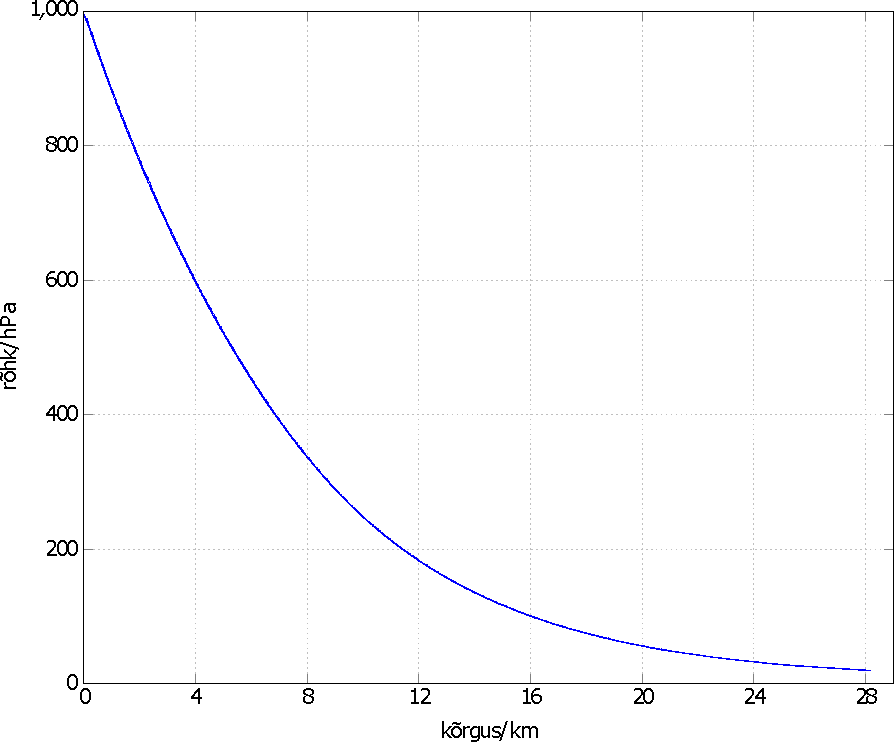
\includegraphics[width=1\textwidth]{PicGra/prekõrg.pdf}
	\caption{Rõhu muutus kõrgusega}
	\allikas{Autori erakogu}
	\label{prekõrg}% Selle järgi viidatakse, see rida peab olema pärast \caption
\end{figure}

Käesolevas osas uuritakse, et kas teooria osas saadud valem, mis kirjeldab rõhu muutust atmosfääris,
\begin{equation*}
p = p_0 \left(1+\frac{\Gamma z}{T_0}\right)^{-\frac{g\mu}{R\Gamma}}
\end{equation*}
vastab katseandmetele. Kuna temperatuuri gradient on erinevatel atmosfääri osades erinev, siis vaatame üksikult osi, kus temperatuuri gradient on konstantne: $g = 9.80665 $ , $R = 8.3144598$ ja $\mu = 0.0289647$. Valemi testimiseks kasutati programmi, mis arvutab algandmete põhjal välja rõhu mõõdetud punkti kõrgusel ja võrdleb sellel kõrgusel mõõdetud rõhuga. Võrdlemise valem on
\begin{equation*}
e = \frac{p_a-p_m}{p_a},
\end{equation*}
kus $p_a$ on arvutatud rõhk ja $p_m$ on mõõdetud rõhk.

Esimene kõrgusevahemik on \SI{22}{m} kuni \SI{793}{m}. Kõrgusel \SI{22}{m} on $p_0=\SI{995.14242}{hPa}$ ja $T_0 = 276.31728$ K. Keskmine erinevus selles kõrgusevahemikus oli \SI{0.515915}{\permil}. Kõrgusel \SI{793}{m} mõõdeti rõhuks \SI{903.92}{hPa} ja arvutati rõhuks \SI{904.276}{hPa}. Järgmise kõrgusvahemikul alguspunktis \SI{808}{m} kõrgusel arvutas programm rõhuks \SI{902.585}{hPa}.

Teine kõrgusevahemik on \SI{808}{m} kuni \SI{2010}{m}. Kõrgusel \SI{808}{m} on $p_0 = 902.01955$ ja $T_0 = 273.510244$ K. Keskmine erinevus selles kõrgusevahemikus oli \SI{0.229426}{\permil}. Kõrgusel \SI{2010}{m} mõõdeti rõhuks \SI{774.026}{hPa} ja arvutati rõhuks \SI{774.777}{hPa}. Järgmise kõrgusvahemikul alguspunktis \SI{2565}{m} kõrgusel arvutas programm rõhuks \SI{721.283}{hPa}. Kui kasutada eelnevas kõrgusvahemikus arvutatud rõhku \SI{808}{m} kõrgusel, mis oli \SI{902.585}{hPa} siis on keskmine erinevus \SI{0.717021}{\permil}. Sellisel juhul on järgmise kõrgusvahemikul alguspunktis \SI{2565}{m} kõrgusel programmi järgi rõhuks \SI{721.735}{hPa}.

Kolmas kõrgusevahemik on \SI{2565}{m} kuni \SI{8154}{m}. Kõrgusel \SI{2565}{m} on $p_0 = 720.86625$ ja $T_0 = 267.189$ K. Keskmine erinevus selles kõrgusevahemikus oli \SI{4.72004}{\permil}. Kõrgusel \SI{8154}{m} mõõdeti rõhuks \SI{329.341}{hPa} ja arvutati rõhuks \SI{332.165}{hPa}. Kui kasutada eelnevas kõrgusvahemikust arvutatud rõhku \SI{2565}{m} kõrgusel, mis oli \SI{721.735}{hPa}, siis on keskmine erinevus \SI{5.91381}{\permil}.

Vaadates langemisel mõõdetud andmeid, on esimene kõrgusvahemik \SI{89}{m} kuni \SI{1926}{m}. Kõrgusel \SI{89}{m} on $p_0=\SI{989.32523}{hPa}$ ja $T_0 = \SI{275.27611}{K}$ ning $\Gamma = \SI{-5.53009}{K/km}$. Keskmine erinevus selles kõrgusevahemikus oli \SI{2.85639}{\permil}. Kõrgusel \SI{1926}{m} mõõdeti rõhuks \SI{786.723}{hPa} ja arvutati rõhuks \SI{784.252}{hPa}. Järgmise kõrgusvahemikul alguspunktis \SI{2136}{m} kõrgusel arvutas programm rõhuks \SI{763.269}{hPa}.

Teisel kõrgusvahemikul \SI{2136}{m} kuni \SI{8154}{m}. Kõrgusel \SI{2136}{m} on $p_0=\SI{765.63645}{hPa}$ ja $T_0 = \SI{265.88365}{K}$ ning $\Gamma = \SI{-7.67992}{K/km}$. Keskmine erinevus selles kõrgusevahemikus oli \SI{4.45647}{\permil}. Kõrgusel \SI{8154}{m} mõõdeti rõhuks \SI{332.17}{hPa} ja arvutati rõhuks \SI{328.404}{hPa}. Kui kasutada eelnevas kõrgusvahemikust arvutatud rõhku \SI{2136}{m} kõrgusel, mis oli \SI{763.269}{hPa}, siis on keskmine erinevus \SI{7.55264}{\permil}.

\section{Mitte adiabaatilised vahemikud}
Atmosfäär ei ole täielikult adiabaatiline. Üks ala, kus atmosfäär ei ole adiabaatiline on pilvedes, kuna pilvedes toimub vee kondenseerumine mille käigus antakse õhule soojusenergiat. Selline protsess toimub umbes \SI{2}{km} kõrgusel nii tõustes kui ka langedes. Visuaalselt on seda võimalik näha jooniselt \ref{tempkõrtrop}. Nüüd arvutatakse välja, kui palju kondenseerub vett umbes \SI{1}{kg} õhu kohta. Selleks kasutatakse teooria osas leitud valemit
\begin{equation*}
\frac{m_v}{m_a} = \frac{i}{2}\frac{R}{\mu L}\left(T_2- T_0 - \Gamma z\right).
\end{equation*}
Tõustes on temperatuurigradient vahetult enne pilvi $\Gamma = \SI{-5.73645}{K/km}$. Temperatuur kõrgusel \SI{2010}{m} on $T_0 = \SI{-6.76}{\degreeCelsius}$ ja sellest $z = \SI{555}{m}$ kõrgemal kõrgusel \SI{2565}{m} on $T_2 = \SI{-7.33}{\degreeCelsius}$. Kasutades valemis katseandmeid saadakse, et õhust eraldub veeauru
\begin{equation*}
\frac{m_v}{m_a} = 0.83 \frac{g}{kg}.
\end{equation*}
Laskudes on temperatuurigradient vahetult enne pilvi $\Gamma = \SI{-5.53009}{K/km}$. Temperatuur kõrgusel \SI{1926}{m} on $T_0 = \SI{-7.81}{\degreeCelsius}$ ja sellest $z = \SI{210}{m}$ kõrgemal kõrgusel \SI{2136}{m} on $T_2 = \SI{-7.88}{\degreeCelsius}$. Kasutades valemis katseandmeid saadakse, et õhust eraldub veeauru
\begin{equation*}
\frac{m_v}{m_a} = 0.16 \frac{g}{kg}.
\end{equation*}

Ka stratosfääris pole atmosfäär adiabaatiline, sest siseenergat antakse õhule juurde päikesest tuleva kiirgusenergiana. Seda on visuaalselt näha jooniselt \ref{TempKõrgus}, kus alates umber \SI{8}{km}'ist alates temperatuur kasvab. Nüüd arvutatakse, kui palju oleks erinevus õhu siseenergias kui päike ei paiskaks. Selleks kasutatakse teooria osas leitud valemit:
\begin{equation*}
\frac{U_2}{U_1} = \frac{T_2}{T_0+\Gamma z}.
\end{equation*}
Temperatuur kõrgusel \SI{8154}{m} on $T_0 = \SI{224.21}{K}$ ja sellest $z = \SI{18753}{m}$ kõrgemal kõrgusel \SI{26907}{m} on $T_2 = \SI{238.6}{k}$. See kõrgus valiti, sest see on viimane lokaalne miinimum õhupalli tõustes ja seega viimane võimalikult täpne õhu temperatuur. Seega, kui päike paistab, on siseenergia 
\begin{equation*}
\frac{U_2}{U_1} = 2.69
\end{equation*}
korda suurem, võrreldes olukorraga kui päikest ei paistaks.

Need arvutused on hinnangulised näitamaks, et atmosfäär ei ole adiabaatiline pilvede sees ja stratosfääris.


\section{Järeldus}






%\cite{book:1339577}

\nocite{*}
%\printbibliography

\appendix% Lisad
\chapter{Andmete analüüsi kood}
\scriptsize
\lstinputlisting[language=C++,breaklines]{Lisad/analüüs.cpp}
\normalsize

\chapter{logifail}
\scriptsize
\lstinputlisting{Lisad/log.txt}
\normalsize


\kinnitusleht% Kinnitusleht
\end{document}
